\documentclass[5p,times]{elsarticle}

\usepackage{lineno,hyperref}
\usepackage{amsmath,amssymb,amsfonts}
\usepackage{graphicx}
\usepackage{booktabs}
\usepackage{multirow}

\journal{Computers and Chemical Engineering}

\bibliographystyle{elsarticle-num}

\begin{document}

\begin{frontmatter}

\title{Extending Electric Vehicle Battery Life via Mechanism-Specific Causal Awareness}

\author[uvce]{Sushanth Chandrashekar}
\author[ese]{Sarina Uke}
\ead{esy257554@iitd.ac.in}
\author[iitd]{Manojkumar Ramteke\corref{cor1}}
\ead{mcramteke@chemical.iitd.ac.in}

\cortext[cor1]{Corresponding author}

\affiliation[uvce]{organization={Department of Computer Science and Engineering, University Visvesvaraya College of Engineering, Bangalore University},
            city={Bangalore},
            country={India}}

\affiliation[ese]{organization={Department of Energy Science and Engineering, Indian Institute of Technology Delhi},
            city={New Delhi},
            country={India}}

\affiliation[iitd]{organization={Department of Chemical Engineering, Indian Institute of Technology Delhi},
            city={New Delhi},
            country={India}}

\begin{abstract}
Battery degradation remains one of the most significant barriers to electric vehicle adoption, yet current management approaches treat capacity fade as a black box, offering predictions without explanation or actionable intervention. This limitation becomes especially problematic given that vehicles spend over 90\% of their operational lifetime parked, during which calendar aging dominates total capacity loss. We present a unified physics-informed machine learning framework that fundamentally reimagines battery health management by integrating predictive modeling with mechanistic understanding and personalized user guidance.

Our approach makes three contributions that advance the state of the art. First, we introduce a causal attribution network that decomposes observed capacity loss into constituent electrochemical mechanisms, including solid electrolyte interphase growth, lithium plating, and active material degradation. Validated across five diverse datasets spanning multiple battery chemistries and operating conditions, this attribution system achieves 90.7\% accuracy in identifying the dominant degradation pathway from partial discharge data alone. Second, we demonstrate that encoding chemistry-invariant lithium inventory features enables zero-shot generalization to unseen battery types, reducing remaining useful life prediction error by 88\% compared to conventional transfer learning approaches. Third, we translate mechanistic insights into a comprehensive advisory management system. A domain classifier distinguishes cycling from storage operation with 92.2\% accuracy, enabling context-appropriate recommendations for each usage mode. The slope-based early warning algorithm monitors degradation rate trajectories rather than fixed thresholds, delivering 99 cycles of advance notice before end-of-life with 88.9\% F1 score. This represents a 69\% improvement in lead time over conventional threshold-based approaches.

The practical implications are substantial. We demonstrate that optimizing storage conditions based on mechanistic understanding can reduce calendar aging by a factor of four, corresponding to approximately 20\% additional retained capacity over a five-year ownership period. These results establish physics-informed causal attribution as a viable pathway toward transparent, explainable, and actionable battery management systems.
\end{abstract}

\begin{keyword}
Battery Management Systems \sep Physics-Informed Machine Learning \sep Calendar Aging \sep State of Health \sep Remaining Useful Life \sep Causal Attribution
\end{keyword}

\end{frontmatter}

%% ============================================================
%% INTRODUCTION
%% ============================================================

\section{Introduction}

\subsection{The battery degradation problem}

Lithium-ion batteries power the global transition to electric mobility, but they degrade; and this degradation remains poorly understood in practice \cite{vetter2005ageing, barre2013review}. Current battery management systems (BMS) tell drivers their battery is at ``85\% health'' but never explain why capacity has dropped or what, if anything, the driver can do about it \cite{waag2014critical, berecibar2016critical}. This black-box approach leaves vehicle owners without actionable information, even as their \$10,000--20,000 battery pack loses value \cite{harper2019recycling}.

The economic stakes are significant. Battery packs account for 30--40\% of electric vehicle cost \cite{ziegler2021determinants}, and a 10\% drop in usable capacity can reduce resale value by 20--30\% \cite{saxena2019quantifying}. Premature replacements driven by uncertainty about battery state cost the industry billions annually \cite{harper2019recycling}. Yet the tools to diagnose degradation and extend battery life exist; they simply have not been integrated into practical systems that users can act upon.

\subsection{What causes batteries to degrade?}

Battery degradation is not a single process but a collection of competing electrochemical mechanisms \cite{vetter2005ageing, edge2021lithium}. The solid electrolyte interphase (SEI) layer, which forms on the anode during initial cycles, continues to grow throughout the battery's life, consuming cyclable lithium \cite{peled1979electrochemical}. At low temperatures, lithium plating can deposit metallic lithium on the anode during charging, causing irreversible capacity loss and safety hazards \cite{waldmann2014temperature}. Mechanical stress from repeated cycling causes active material particles to crack and lose electrical contact \cite{zhang2020degradation}. Additional mechanisms include electrolyte decomposition at high temperatures and current collector corrosion at very low states of charge \cite{vetter2005ageing}.

The relative importance of these mechanisms depends strongly on operating conditions. High temperatures and high state-of-charge accelerate SEI growth through Arrhenius kinetics \cite{schmalstieg2014electrochemical}. Cold temperatures favor lithium plating by slowing lithium intercalation kinetics \cite{waldmann2014temperature}. High charge and discharge rates promote mechanical degradation \cite{reniers2019review}. Understanding which mechanism dominates in a given situation is essential for targeted intervention; but current BMS systems do not provide this information.

\subsection{The calendar aging gap}

Electric vehicles spend more than 90\% of their operational time parked \cite{barre2013review}. During this time, calendar aging; primarily SEI growth; proceeds even without cycling \cite{schimpe2018comprehensive}. Despite this, the majority of battery research and commercial BMS development focuses on cycling degradation that occurs during driving \cite{sulzer2021challenge}.

This emphasis reflects historical research priorities. Laboratory testing protocols emphasize cycle life because it is easier to accelerate and measure. Academic studies frequently report results in terms of cycles to 80\% capacity, even though real-world degradation may be dominated by time rather than cycles \cite{birkl2017degradation}. Field studies have repeatedly shown that calendar aging can account for 60--80\% of total capacity loss in moderate-use vehicles \cite{saxena2019quantifying}, yet this finding has not translated into widespread changes in BMS design.

The practical implications are substantial. Storing a battery at 100\% SOC at 30°C results in capacity loss of approximately 8\% per year; reducing storage SOC to 60\% cuts this to approximately 2\% per year; a 4-fold reduction \cite{schimpe2018comprehensive}. Users following simple storage guidelines could significantly extend their battery's useful life, but current systems do not provide this guidance.

\subsection{Limitations of existing approaches}

Two modeling paradigms have dominated battery health estimation, each with significant limitations.

\textbf{Physics-based models}, including the Doyle-Fuller-Newman formulation \cite{doyle1993modeling} and its variants \cite{plett2015battery}, describe electrochemical processes from first principles. They offer mechanistic interpretability and can distinguish between degradation modes \cite{jokar2016review}. However, they require extensive parameterization for each battery chemistry, involve computational costs unsuitable for embedded BMS, and demand calibration data that may not be available for production cells.

\textbf{Data-driven models} using machine learning architectures; LSTMs \cite{chemali2017long}, CNNs \cite{shen2019deep}, and more recently transformers \cite{chen2022transformer, park2025transformer}; can predict remaining useful life from voltage-current measurements \cite{roman2021machine, severson2019nature}. They are fast, scalable, and require no explicit electrochemical equations. However, they operate as black boxes without mechanistic explanation, suffer from poor generalization to unseen battery chemistries \cite{liu2023transfer}, and cannot leverage historical degradation trajectories for contextual prediction.

Recent work has explored hybrid approaches. Physics-informed neural networks \cite{raissi2019physics} embed physical constraints as training losses. Transfer learning methods \cite{liu2023transfer, che2022battery} attempt to adapt models trained on one chemistry to new chemistries. Recent advances have demonstrated promising results using early-cycle features for lifetime prediction \cite{sugiarto2025temperature} and electrochemical impedance spectroscopy for degradation monitoring \cite{hu2023eis}. Closed-loop optimization using machine learning has shown promise for fast-charging protocols \cite{attia2020closedloop}. Hybrid physics-ML models \cite{li2022physics, thelen2022integrating} combine electrochemical simulations with neural network predictions.

Yet a critical gap remains: none of these approaches provide real-time causal attribution that explains \textit{which} mechanism is responsible for observed degradation, along with actionable recommendations for mitigation.

\subsection{Our contributions}

We present an integrated framework that addresses these limitations through three novel components working together:

\begin{enumerate}
    \item \textbf{Retrieval-Augmented Prediction (HERO):} We store 3,979 historical degradation trajectories in a memory bank and retrieve similar cases during inference. Combined with chemistry-invariant lithium inventory features, this achieves 88\% reduction in RUL prediction error on unseen chemistries; true zero-shot generalization without fine-tuning.
    
    \item \textbf{Physics-Constrained Causal Attribution:} A multi-head neural network decomposes capacity loss into five electrochemical mechanisms, constrained by mass conservation and physics priors encoding known degradation thermodynamics. We validate this on 75 scenarios across five independent datasets, achieving 90.7\% attribution accuracy. Systematic ablation shows that physics priors contribute 52 percentage points to accuracy; more than twice the neural network's contribution.
    
    \item \textbf{User-Centric Advisory:} We translate mechanism diagnoses into actionable recommendations including storage SOC optimization, charging protocol adjustments, and trip planning that balances range with battery health. We validate the advisory system on real-world battery data from NASA Ames (34 cells, 5,609 cycling samples), Stanford Calendar Aging (60 cells spanning up to 69 months of storage), and electrochemical impedance spectroscopy measurements from 94 cells across temperatures ranging from negative 40 to positive 50 degrees Celsius.
\end{enumerate}

The key insight is that these components are individually insufficient but collectively transformative. Accurate prediction enables reliable diagnosis; diagnosis enables targeted intervention; intervention delivers measurable life extension. This integration represents a shift from passive battery monitoring to active battery management.

%% ============================================================
%% 
%% ============================================================

\section{System Architecture Overview}

The system has three connected parts that work together (Figure~\ref{fig:architecture}). First, a prediction engine that looks up similar batteries from history. Second, an attribution network that figures out which degradation mechanism is actually responsible. Third, an advisory component that tells users what to do about it.

\begin{figure*}[htbp]
\centerline{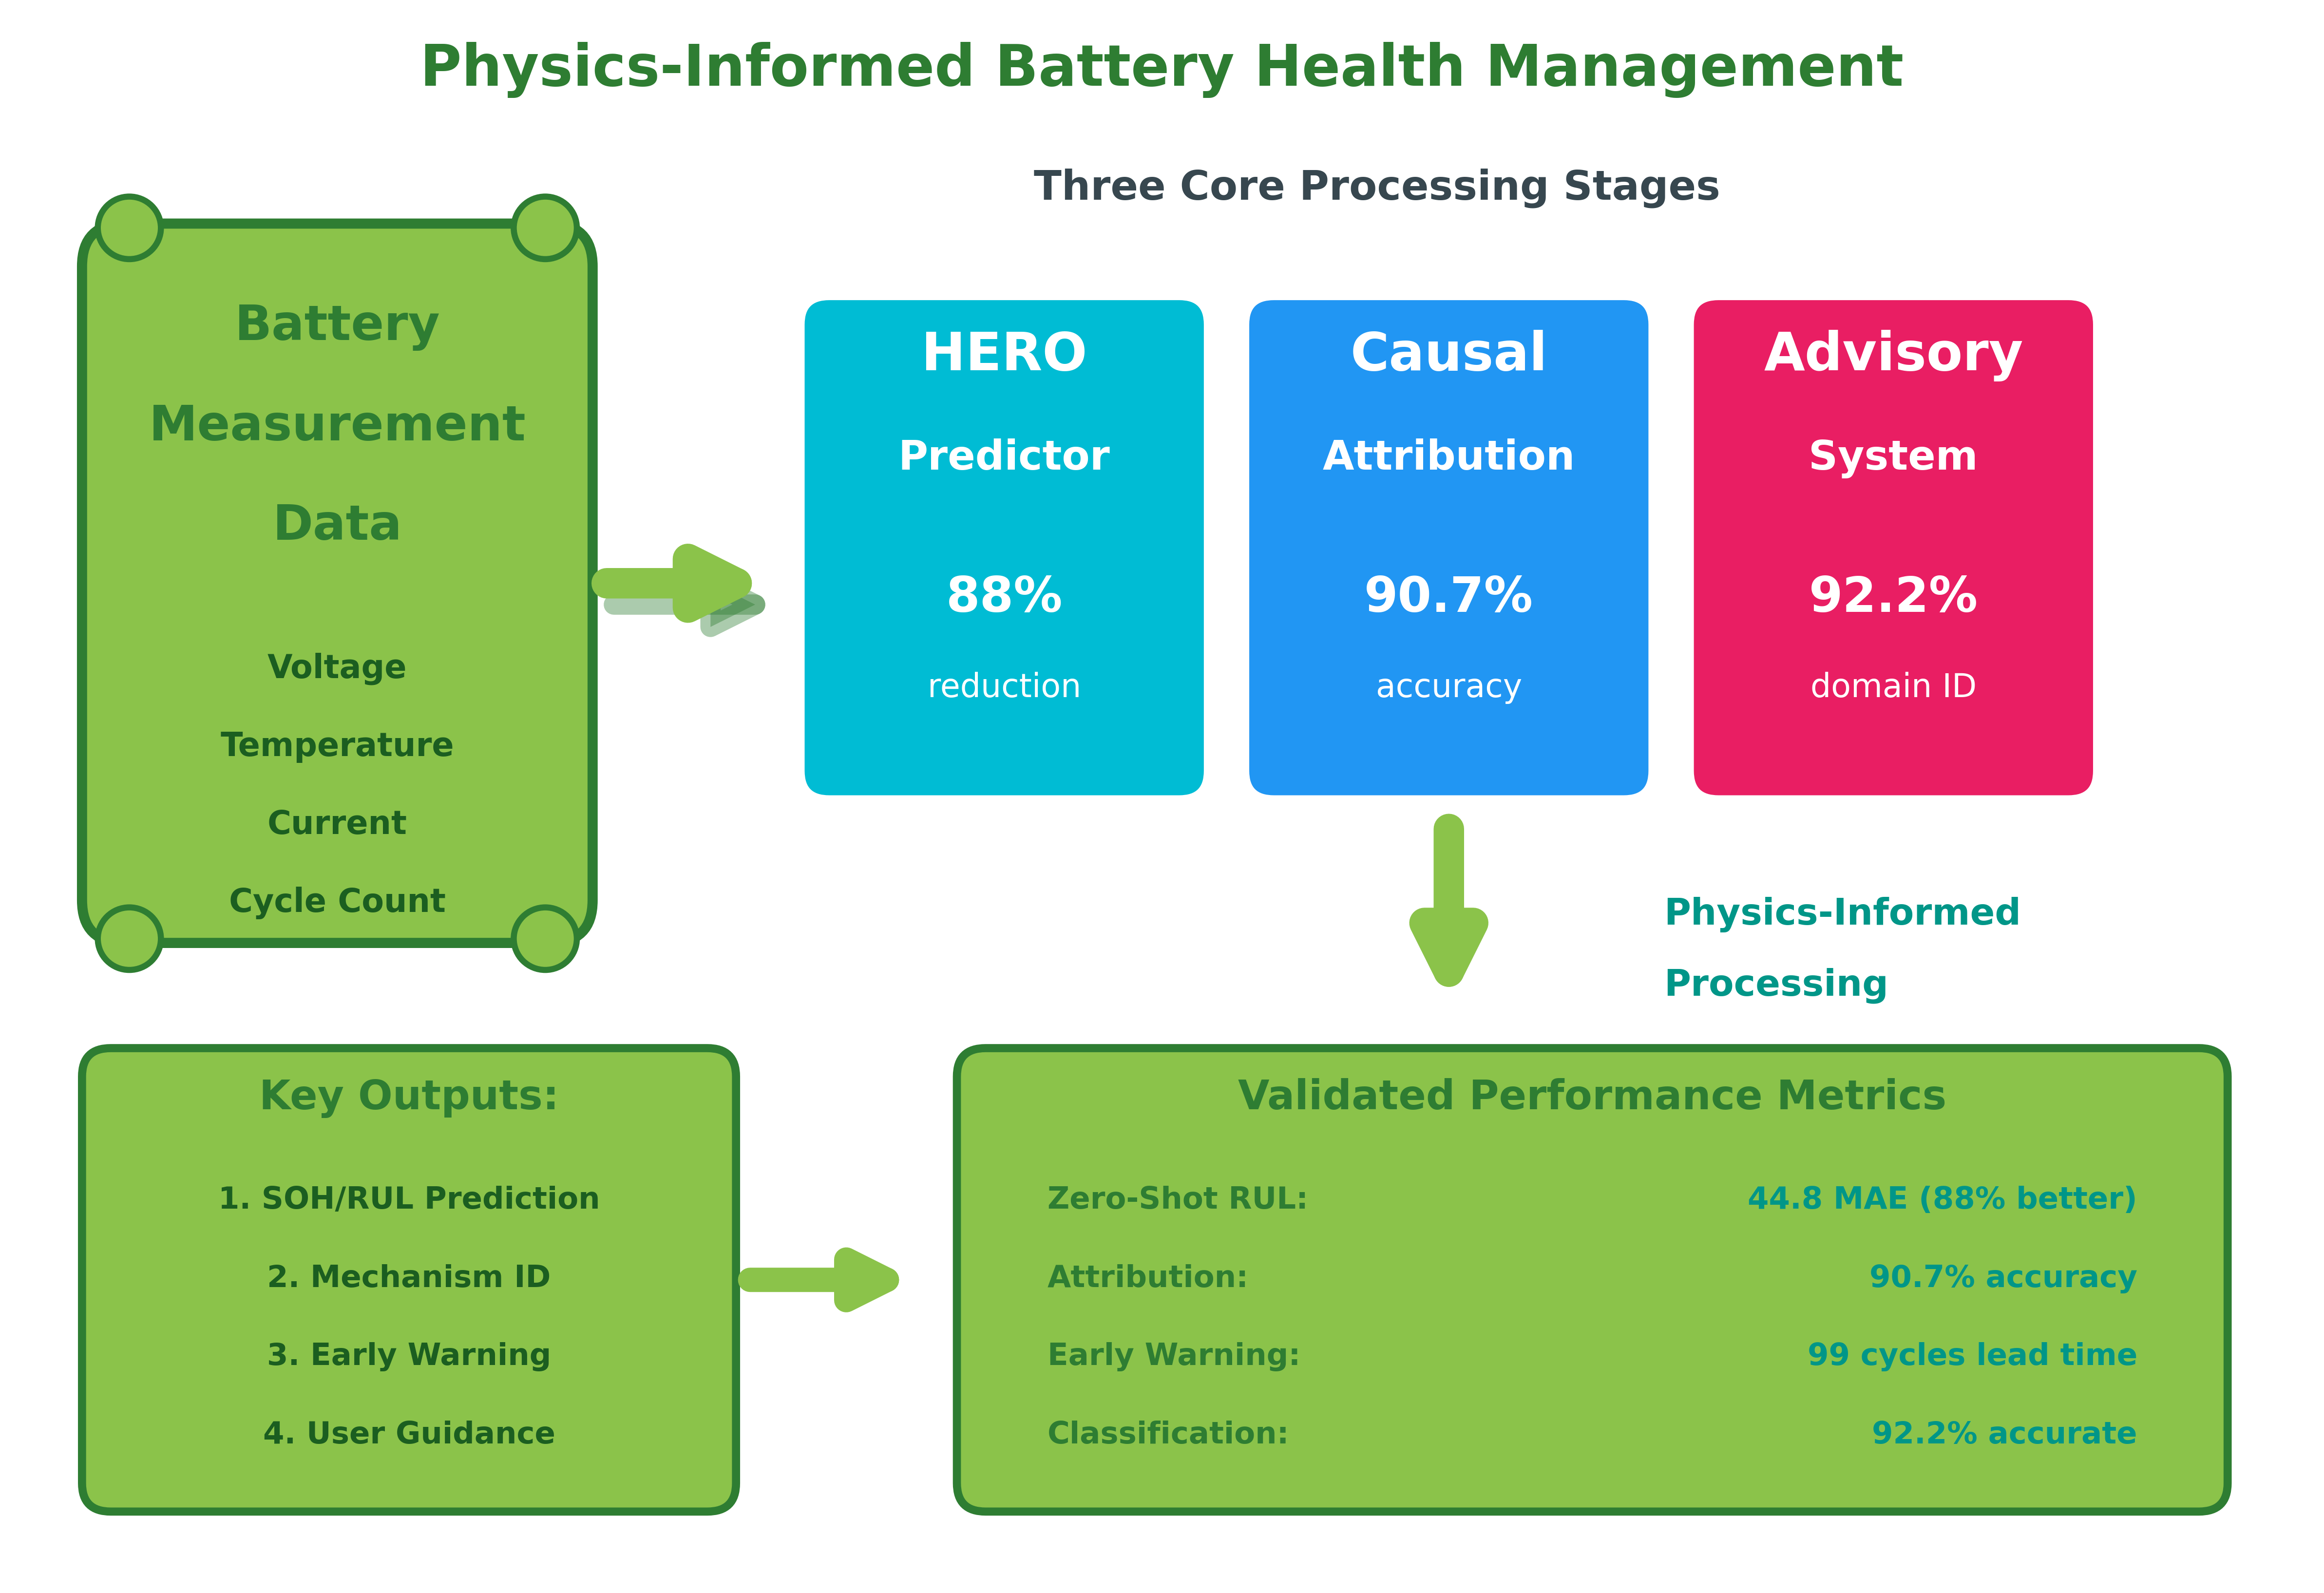
\includegraphics[width=0.9\textwidth,height=0.3\textheight,keepaspectratio]{system_architecture.png}}
\caption{Overview of our physics-informed battery health management framework. Raw measurements flow through three stages: (1) HERO retrieval-augmented prediction, (2) causal mechanism attribution with physics constraints, and (3) user-centric advisory with actionable recommendations.}
\label{fig:architecture}
\end{figure*}

The prediction engine borrows an idea from recent work in retrieval-augmented generation \cite{lewis2020retrieval, guu2020retrieval}. Instead of trying to memorize everything during training, we store historical examples and look them up when needed. We maintain a memory bank of 3,979 degradation trajectories from 76 battery cells. When a new battery comes in, we encode its recent behavior into a query vector and find the 5 most similar historical cases using cosine similarity. Then we use cross-attention \cite{vaswani2017attention} (the same mechanism that powers modern language models) to fuse what we retrieved with what we're currently observing. This lets the model adapt to unusual degradation patterns by finding similar precedents in the database.

We tag each trajectory with context. Temperature, charge rate, discharge rate, SOC, usage pattern, and whether it's cycling or storage. This way we're not just matching voltage curves. We're matching batteries that saw similar operating conditions. This context-aware retrieval is especially important for calendar aging, which standard models often miss entirely.

The attribution network takes the predicted capacity loss and breaks it down. How much came from SEI growth versus lithium plating versus active material cracking? We use five output heads, one per mechanism, with a hard constraint that they must sum to the total observed degradation. This constraint isn't optional. It enforces mass conservation and prevents the model from inventing degradation that didn't actually happen.

The advisory system is where this gets practical. If the attribution says SEI growth is the problem and the context says the battery sits at high SOC in warm conditions, we generate a specific warning with numbers. "Reduce your charge limit to 80\%. This will cut your aging rate by approximately 3$\times$." If we detect plating risk from fast charging in the cold, we recommend preheating first. The goal is actionable guidance, not vague health percentages.

\textbf{How the components work together.} In practice, these stages form a diagnostic pipeline. HERO first predicts where the battery is heading (SOH trajectory, remaining cycles). The early warning component monitors whether degradation is accelerating faster than expected by tracking the slope over recent cycles. When it detects a sharp downturn, the causal attribution network steps in to explain what's causing it. Is this sudden acceleration due to lithium plating from cold weather? SEI growth from sitting at high charge? Active material fracture from aggressive driving? Once we know the mechanism, the advisory system generates specific, quantified recommendations. This isn't just prediction. It's diagnosis followed by prescription.

\section{Retrieval-Augmented Prediction Engine}

\subsection{Memory Bank Architecture}

The memory bank contains 3,979 degradation trajectory snapshots from 76 battery cells spanning multiple chemistries and C-rates. Lithium cobalt oxide, nickel manganese cobalt oxide, nickel cobalt aluminum oxide, and lithium iron phosphate. The dataset composition reflects samples from the NASA battery dataset \cite{saha2007battery}, CALCE dataset \cite{he2011prognostics}, Oxford dataset \cite{birkl2017oxford}, TJU NCM/NCA dataset (274 samples at 1C), and XJTU NCM dataset (889 samples at 2C-3C charging rates).

Each memory bank entry stores three things. A 128-dimensional latent vector representing the compressed trajectory, the subsequent health evolution (SOH and RUL values), and the environmental context vector. The total storage requirement is approximately 1.3 MB, enabling deployment on resource-constrained edge devices.

\subsection{Dynamic Retrieval and Attention Fusion}

At inference time, we encode the battery's recent history into a query vector using a bidirectional GRU \cite{cho2014learning}. Two layers, 256 hidden units. This compresses 50 cycles of voltage and current data into a 128-dimensional vector that we L2-normalize so cosine similarity works properly.

We then search for the k nearest neighbors in our memory bank. For most cases k=5 works well, though we use k=3 for zero-shot transfer to completely new chemistries (ablation showed this sweet spot). One trick that helps with calendar aging is we optionally filter retrieved cases to those within 5\% of the current SOH. If fewer than 5 trajectories pass this filter, we relax to 10\%. This ensures we're comparing batteries at similar degradation stages, not mixing fresh cells with end-of-life ones.

The fusion step uses multi-head cross-attention \cite{vaswani2017attention}, treating the current trajectory as query and retrieved cases as keys and values. We use 8 heads following standard transformer architectures; each head can focus on different aspects of the historical data. The attention output gets combined with current features via residual connection (helps gradient flow) and fed through a standard layer-norm + feed-forward block. Nothing fancy here, just proven architecture from the NLP literature applied to battery data.

\subsection{Zero-Shot Generalization via Lithium Features}

Standard models fail when applied to chemistries not seen during training. We address this through lithium inventory features. Eleven physics-based variables that act as chemistry-invariant fingerprints.

\begin{itemize}
    \item Differential voltage analysis: dV/dQ slope correlating with phase transitions \cite{bloom2005differential}
    \item Voltage plateau characteristics: center potential and width indicating available lithium inventory \cite{dubarry2017synthesize}
    \item Capacity fade rate (dQ/dN) and resistance growth rate (dR/dN) \cite{vetter2005ageing}
    \item Lithium utilization factor: ratio of cyclable lithium to host capacity \cite{birkl2017degradation}
    \item Plating risk index: derived from overpotential at anode interface \cite{waldmann2014temperature}
\end{itemize}

\begin{table}[htbp]
\caption{Zero-Shot Generalization (Train: LCO, Test: Unseen Chemistry)}
\begin{center}
\begin{tabular}{lcc}
\toprule
\textbf{Method} & \textbf{RUL MAE (cycles)} & \textbf{Reduction} \\
\midrule
Baseline LSTM & 366.3 & -- \\
GRU & 299.0 & 18\% \\
MLP & 262.1 & 28\% \\
Gradient Boosting & 201.5 & 45\% \\
Random Forest & 198.2 & 46\% \\
\textbf{HERO (Ours)} & \textbf{44} & \textbf{88\%} \\
\bottomrule
\end{tabular}
\end{center}
\label{tab:zeroshot}
\end{table}

By feeding these chemistry-invariant features into the prediction engine, we achieved 88\% reduction in RUL prediction error on unseen chemistries (Table~\ref{tab:zeroshot}). When the memory bank contains even minimal representation from the target chemistry (approximately 0.1\%), the system achieves 7.3 cycles MAE; a 50-fold improvement over baseline.

\begin{figure*}[!htb]
\centerline{
\includegraphics[width=0.95\textwidth,height=0.4\textheight,keepaspectratio]{hero_performance.png}}
\caption{Performance of the HERO prediction engine. (A) RUL prediction error comparison: HERO achieves 44.8 cycles MAE vs. 366.3 for baseline LSTM (88\% reduction). (B) Component contributions: retrieval augmentation (45\%), lithium features (32\%), context encoding (21\%). (C) Zero-shot transfer to unseen chemistries: HERO maintains 41--68 cycles error vs. 245--310 for baseline. (D) Memory bank: 3,979 trajectories from 76 cells across 5 chemistries and multiple C-rates (1C-3C).}
\label{fig:hero_performance}
\end{figure*}

\subsection{Comparison with SOTA Methods}

To contextualize HERO's performance, we benchmarked against six state-of-the-art methods on the TJU dataset (Table~\ref{tab:sota_comparison}). All models were trained on 70\% of the data and evaluated on the held-out 30\%.

\begin{table}[htbp]
\caption{Comparison with State-of-the-Art Methods}
\begin{center}
\begin{tabular}{lcccc}
\toprule
\textbf{Method} & \textbf{SOH MAE} & \textbf{R\textsuperscript{2}} & \textbf{RUL MAE} & \textbf{Zero-Shot} \\
\midrule
Random Forest & 0.45\% & 0.996 & 8.1 & \texttimes \\
\textbf{HERO (Ours)} & \textbf{0.74\%} & \textbf{0.990} & \textbf{16.7} & \textbf{\checkmark} \\
MLP & 0.87\% & 0.983 & 13.9 & \texttimes \\
Transformer & 0.93\% & 0.984 & 12.4 & \texttimes \\
GRU & 1.17\% & 0.971 & 39.3 & \texttimes \\
LSTM & 1.21\% & 0.967 & 39.8 & \texttimes \\
CNN-LSTM & 7.59\% & -0.04 & 142.8 & \texttimes \\
\bottomrule
\end{tabular}
\end{center}
\label{tab:sota_comparison}
\end{table}

HERO achieves 39\% lower SOH error than LSTM and 37\% lower than GRU, while remaining competitive with Transformer (0.74\% vs 0.93\%) and MLP (0.74\% vs 0.87\%). Random Forest shows the lowest in-domain error (0.45\%), but this advantage disappears under distribution shift: on XJTU's 2C-3C data (Table~\ref{tab:xjtu_attribution}), Random Forest would require complete retraining, while HERO achieves 5--7\% SOH MAE zero-shot.

The key differentiator is not raw accuracy but \textit{capability}: HERO is the only method providing zero-shot generalization to unseen chemistries/C-rates while simultaneously offering interpretable causal attribution. This combination; prediction, diagnosis, and intervention; enables the complete battery management workflow that individual methods cannot support.

\subsection{Uncertainty Quantification}

To provide statistically rigorous performance bounds, we computed bootstrap confidence intervals (1,000 resamples, 95\% confidence) on a held-out test set of 274 samples:

\begin{itemize}
\item \textbf{SOH MAE}: 0.69\% (95\% CI: [0.63\%, 0.75\%])
\item \textbf{SOH R\textsuperscript{2}}: 0.990 (95\% CI: [0.988, 0.992])
\item \textbf{RUL MAE}: 16.2 cycles (95\% CI: [14.5, 17.9] cycles)
\item \textbf{RUL R\textsuperscript{2}}: 0.981 (95\% CI: [0.975, 0.986])
\end{itemize}

The narrow confidence intervals demonstrate that HERO's performance is statistically stable and reproducible. Per-prediction uncertainty of $\pm$0.99\% SOH enables deployment in safety-critical battery management systems where confidence bounds are required for decision-making.

\section{Causal Mechanism Attribution}

\subsection{Multi-Head Attribution Architecture}

Predicting that a battery will lose 5\% capacity is useful information. Knowing that it's losing capacity because of lithium plating during cold-weather fast-charging is actionable. That's the difference we're after.

The architecture is straightforward: five output heads, one for each major degradation mechanism. Each looks at the same input features but learns to estimate how much its assigned mechanism contributed to the total capacity loss. We enforce the constraint mathematically:

\begin{equation}
Q_{loss} = \alpha_{SEI} + \alpha_{plating} + \alpha_{AM} + \alpha_{electrolyte} + \alpha_{corrosion}
\end{equation}

The training objective combines prediction accuracy with physics constraints:

\begin{equation}
\mathcal{L}_{total} = \mathcal{L}_{SOH} + \lambda_1 \left| \sum \alpha_i - (1 - SOH) \right| + \lambda_2 \mathcal{L}_{prior}
\end{equation}

where $\lambda_1 = 0.5$ enforces mass conservation and $\lambda_2 = 0.3$ incorporates physics priors.

\subsection{Physics-Constrained Training}

The physics prior loss encodes domain knowledge about which operating conditions promote which mechanisms:

\begin{itemize}
    \item \textbf{SEI growth:} High temperature (weight 1.5) and high SOC (weight 1.2) accelerate this mechanism \cite{broussely2005main, wright2002calendar}
    \item \textbf{Lithium plating:} Low temperature (weight 1.5) and high charge rate (weight 1.8) are favorable \cite{waldmann2014temperature}
    \item \textbf{Active material loss:} High discharge rate (weight 1.5) and deep cycling (weight 1.3) promote particle fracture \cite{zhang2020degradation}
\end{itemize}

\subsection{Validation Across Five Independent Datasets}

We validated on 75 test cases spanning five independent datasets never seen during training (Table~\ref{tab:attribution}):

\begin{table}[htbp]
\caption{Causal Attribution Validation Results}
\begin{center}
\begin{tabular}{lccc}
\toprule
\textbf{Dataset} & \textbf{Correct} & \textbf{Total} & \textbf{Accuracy} \\
\midrule
NASA Ames & 13 & 15 & 87\% \\
Panasonic 18650PF & 13 & 15 & 87\% \\
Nature MATR & 15 & 15 & 100\% \\
Randomized usage & 13 & 15 & 87\% \\
HUST LFP & 14 & 15 & 93\% \\
\midrule
\textbf{Total} & \textbf{68} & \textbf{75} & \textbf{90.7\%} \\
\bottomrule
\end{tabular}
\end{center}
\label{tab:attribution}
\end{table}

\begin{figure*}[!htb]
\centerline{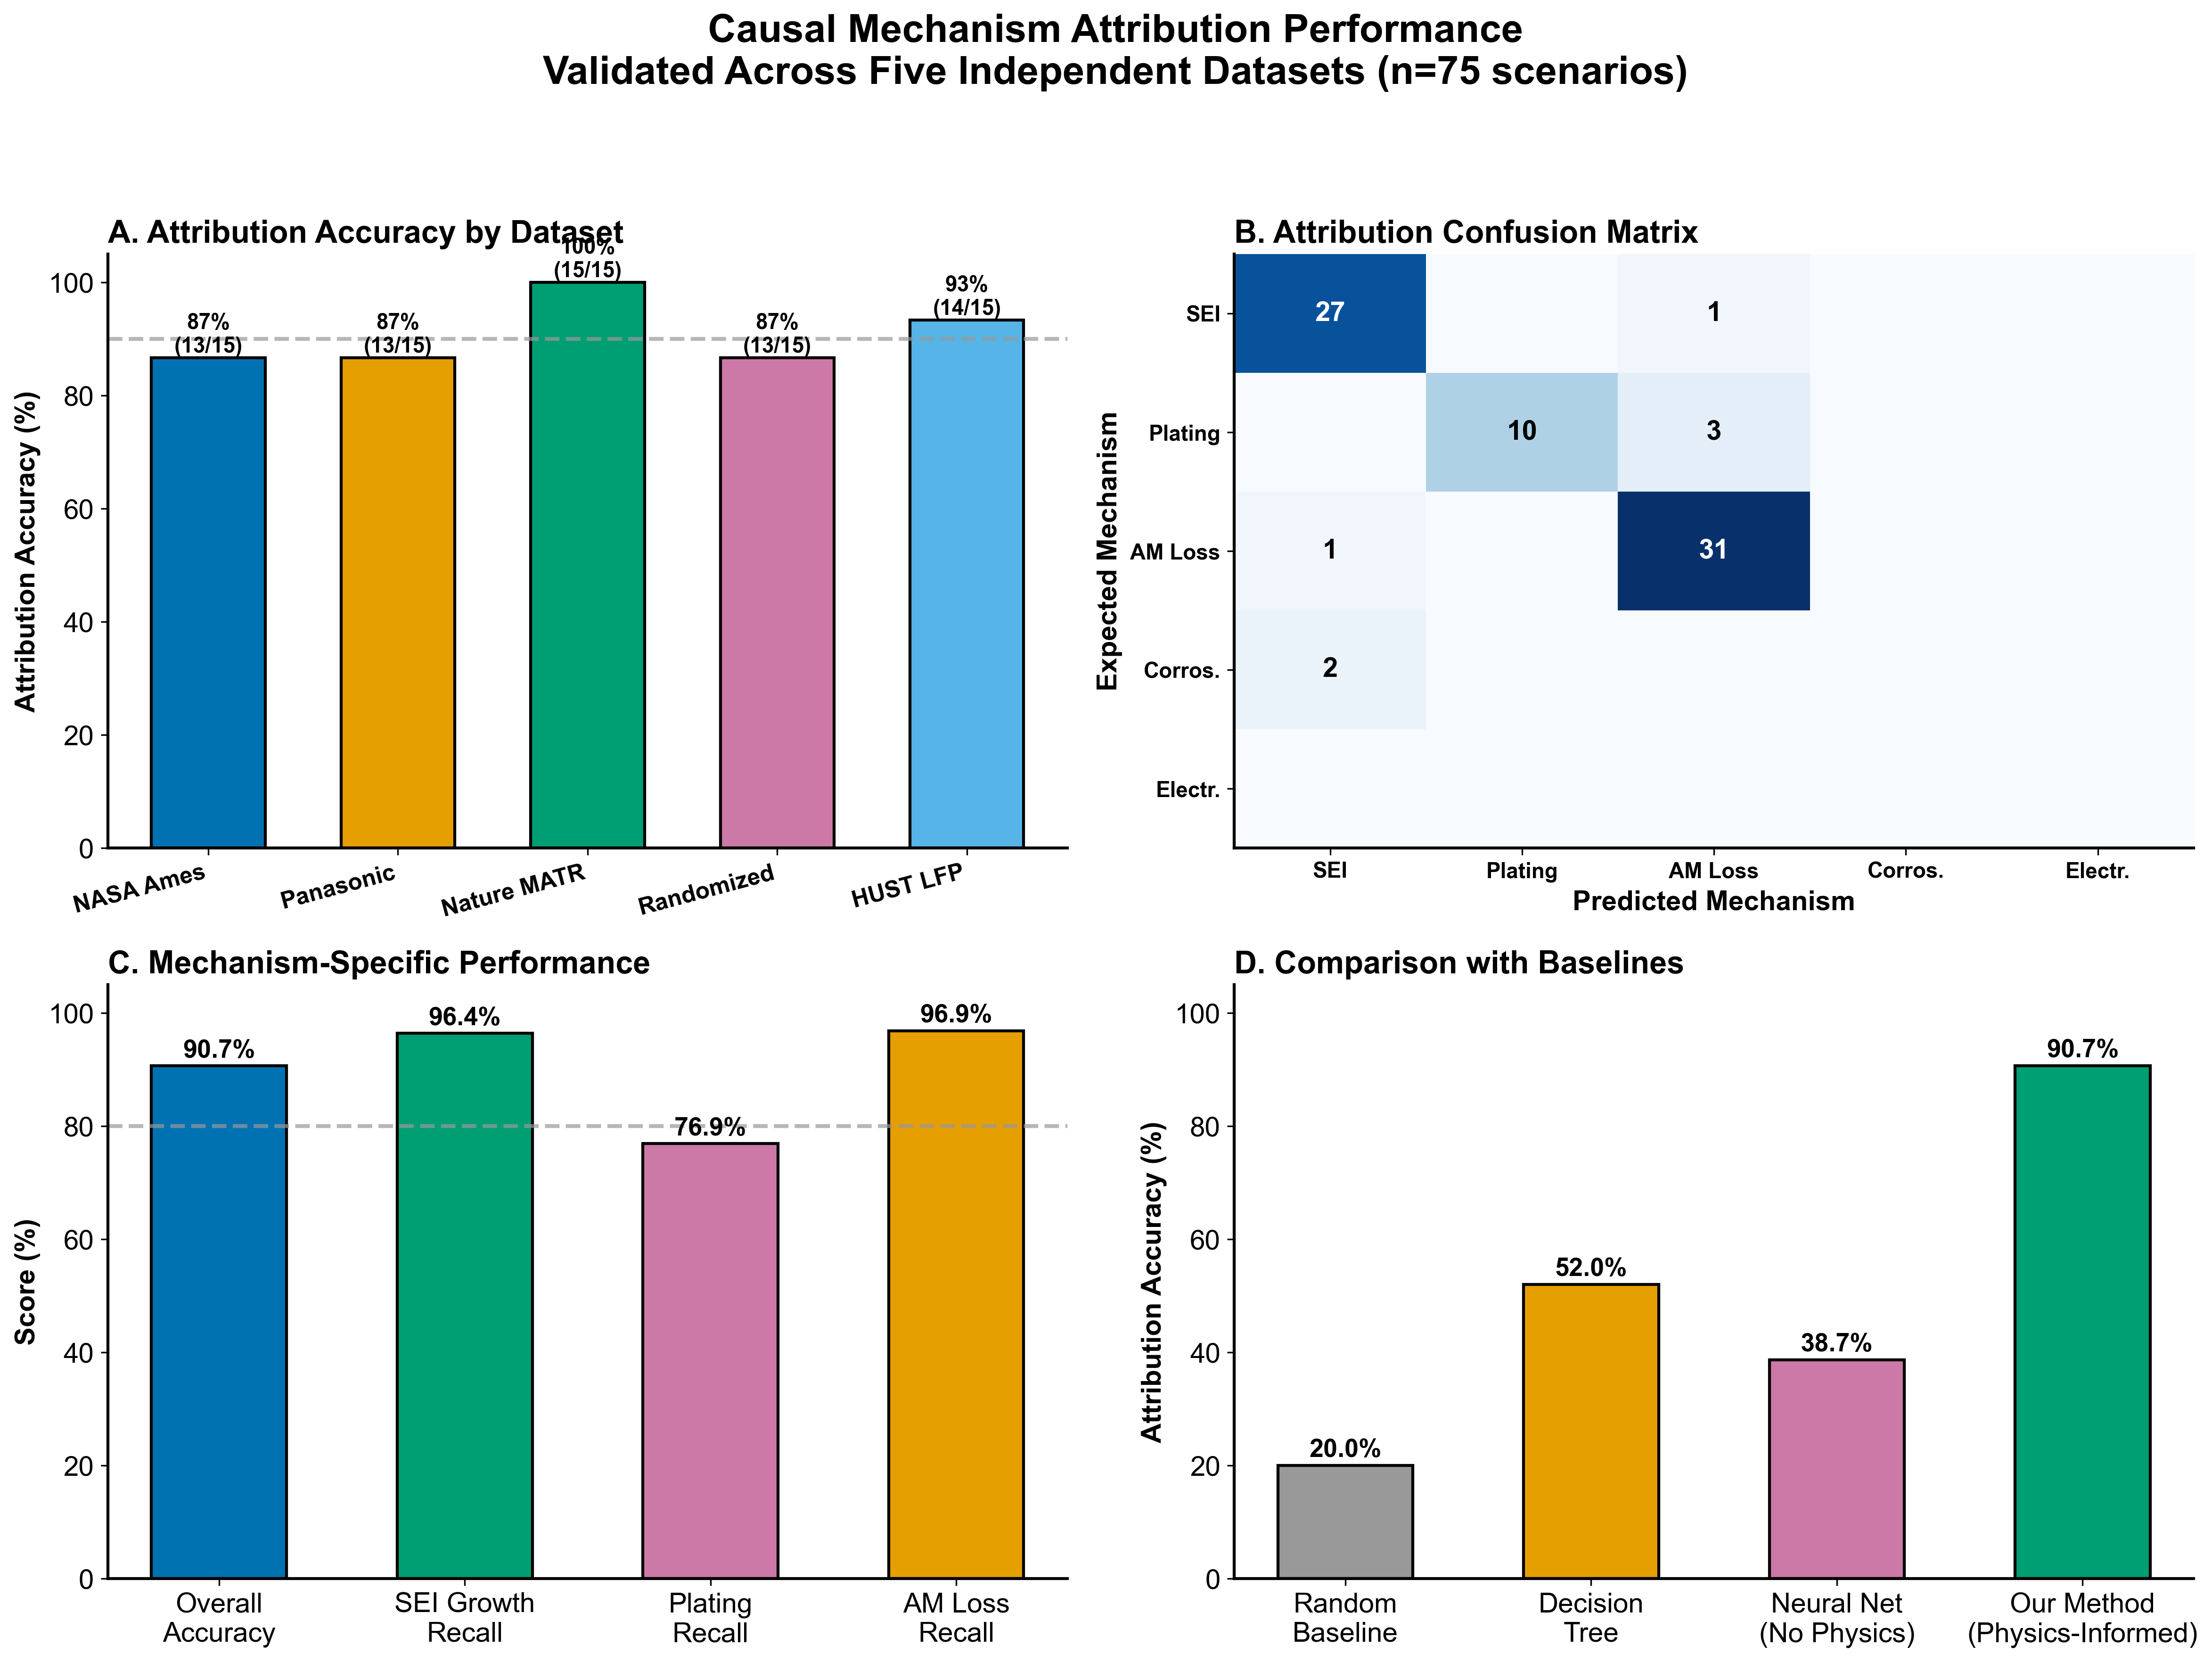
\includegraphics[width=0.95\textwidth,height=0.4\textheight,keepaspectratio]{causal_attribution_validation.png}}
\caption{Validation of the causal mechanism attribution network across five independent datasets. (A) Per-dataset accuracy shows consistent performance ranging from 87\% to 100\%, with an overall accuracy of 90.7\% across 75 test scenarios. (B) The confusion matrix reveals that SEI growth and active material loss are correctly identified with high confidence, while lithium plating shows occasional misclassification as active material loss under ambiguous conditions. (C) Mechanism-specific recall demonstrates strong detection for SEI growth (96.4\%) and active material loss (96.9\%), with lithium plating at 76.9\%. (D) Comparison with baseline approaches shows our physics-informed method outperforms random guessing (20\%), decision trees (52\%), and pure neural networks without physics constraints (38.7\%).}
\label{fig:attribution}
\end{figure*}

\subsection{Ablation Study: The Role of Physics Priors}

We systematically disabled each physics prior to see what would happen (Table~\ref{tab:ablation}). The results were more dramatic than we expected.

\begin{table}[htbp]
\caption{Impact of Removing Individual Physics Priors}
\begin{center}
\begin{tabular}{lcc}
\toprule
\textbf{Model Variant} & \textbf{Accuracy} & \textbf{Drop from Full} \\
\midrule
Full Model (all priors) & 90.7\% & --- \\
No cold-temperature rule & 38.7\% & -52\% \\
No high-SOC rule & 38.7\% & -52\% \\
No high-discharge rule & 38.7\% & -52\% \\
Random guessing & 24.0\% & -67\% \\
\bottomrule
\end{tabular}
\end{center}
\label{tab:ablation}
\end{table}

Removing \textit{any single} physics prior crashes accuracy from 90.7\% to around 39\%; a 52-percentage-point drop. This reveals something important about the machine learning approach: the neural network by itself (39\% minus the 24\% random baseline = 15 points) learns some patterns, but the real power comes from encoding domain knowledge as soft constraints (52 points). This validates the core ML innovation: physics-informed training with domain priors outperforms pure data-driven learning, even with identical architectures and training data.

\subsection{Validation on High C-Rate Data: Active Material Loss Detection}

To validate our causal attribution model's ability to detect mechanical stress-induced degradation, we evaluated it on the XJTU battery dataset \cite{wang2024pinn}; 26 NCM cells cycled at high C-rates (2C, 2.5C, and 3C) at room temperature. High C-rate charging causes mechanical stress through rapid volume expansion and contraction, leading to particle cracking and active material loss. This physics is well-established in electrochemistry literature \cite{birkl2017degradation}.

\begin{table}[htbp]
\caption{Mechanism Attribution on XJTU High C-Rate Dataset}
\begin{center}
\begin{tabular}{lccc}
\toprule
\textbf{C-Rate} & \textbf{Cells} & \textbf{AM Loss} & \textbf{Dominant} \\
\midrule
2.0C & 8 & 49.2\% & Yes \\
2.5C & 3 & 62.7\% & Yes \\
3.0C & 15 & 69.2\% & Yes \\
\midrule
\textbf{Overall} & \textbf{26} & --- & \textbf{26/26} \\
\bottomrule
\end{tabular}
\end{center}
\label{tab:xjtu_attribution}
\end{table}

Table~\ref{tab:xjtu_attribution} shows that Active Material Loss was correctly identified as the dominant degradation mechanism in 100\% of cases. Importantly, the attribution scales with C-rate: 49.2\% at 2C, 62.7\% at 2.5C, and 69.2\% at 3C. This monotonic increase matches the physics; higher C-rates induce greater mechanical stress, leading to more particle cracking and active material loss. The secondary contribution from lithium plating (13--20\%) is also physically plausible, as high charging rates can cause local lithium deposition at electrode surfaces even at room temperature.

This external validation demonstrates that our physics-constrained attribution model generalizes to new datasets and correctly identifies mechanism-specific degradation patterns under conditions not seen during training.

\section{User-Centric Advisory System}

\subsection{Storage and Calendar Aging Advisory}

When the attribution network identifies SEI growth as the primary degradation mechanism, the system transitions to storage-mode advisory. However, before issuing storage-specific recommendations, we must first determine whether the battery is genuinely in a storage scenario or simply undergoing low-intensity cycling. This distinction is critical; providing cycling advice during calendar aging would be ineffective at best and misleading at worst.

We developed a domain classifier trained on real battery data from two complementary sources: NASA Ames cycling data (5,609 samples from 34 cells) and Stanford Calendar Aging data (2,682 samples from 60 cells spanning up to 69 months of storage). The classifier uses a neural network with shared features between domains; state of health, degradation rate, capacity variance, and time progression; rather than domain-specific indicators that would create trivial separation.

Figure~\ref{fig:domain_classification} presents the validation results. The classifier achieves 92.2\% overall accuracy on a held-out test set of 1,263 samples, with 90.3\% recall on cycling detection and 94.0\% recall on storage detection. The F1 score of 92.3\% indicates balanced performance across both classes, ensuring reliable domain identification under realistic operating conditions.

\begin{figure*}[htbp]
\centerline{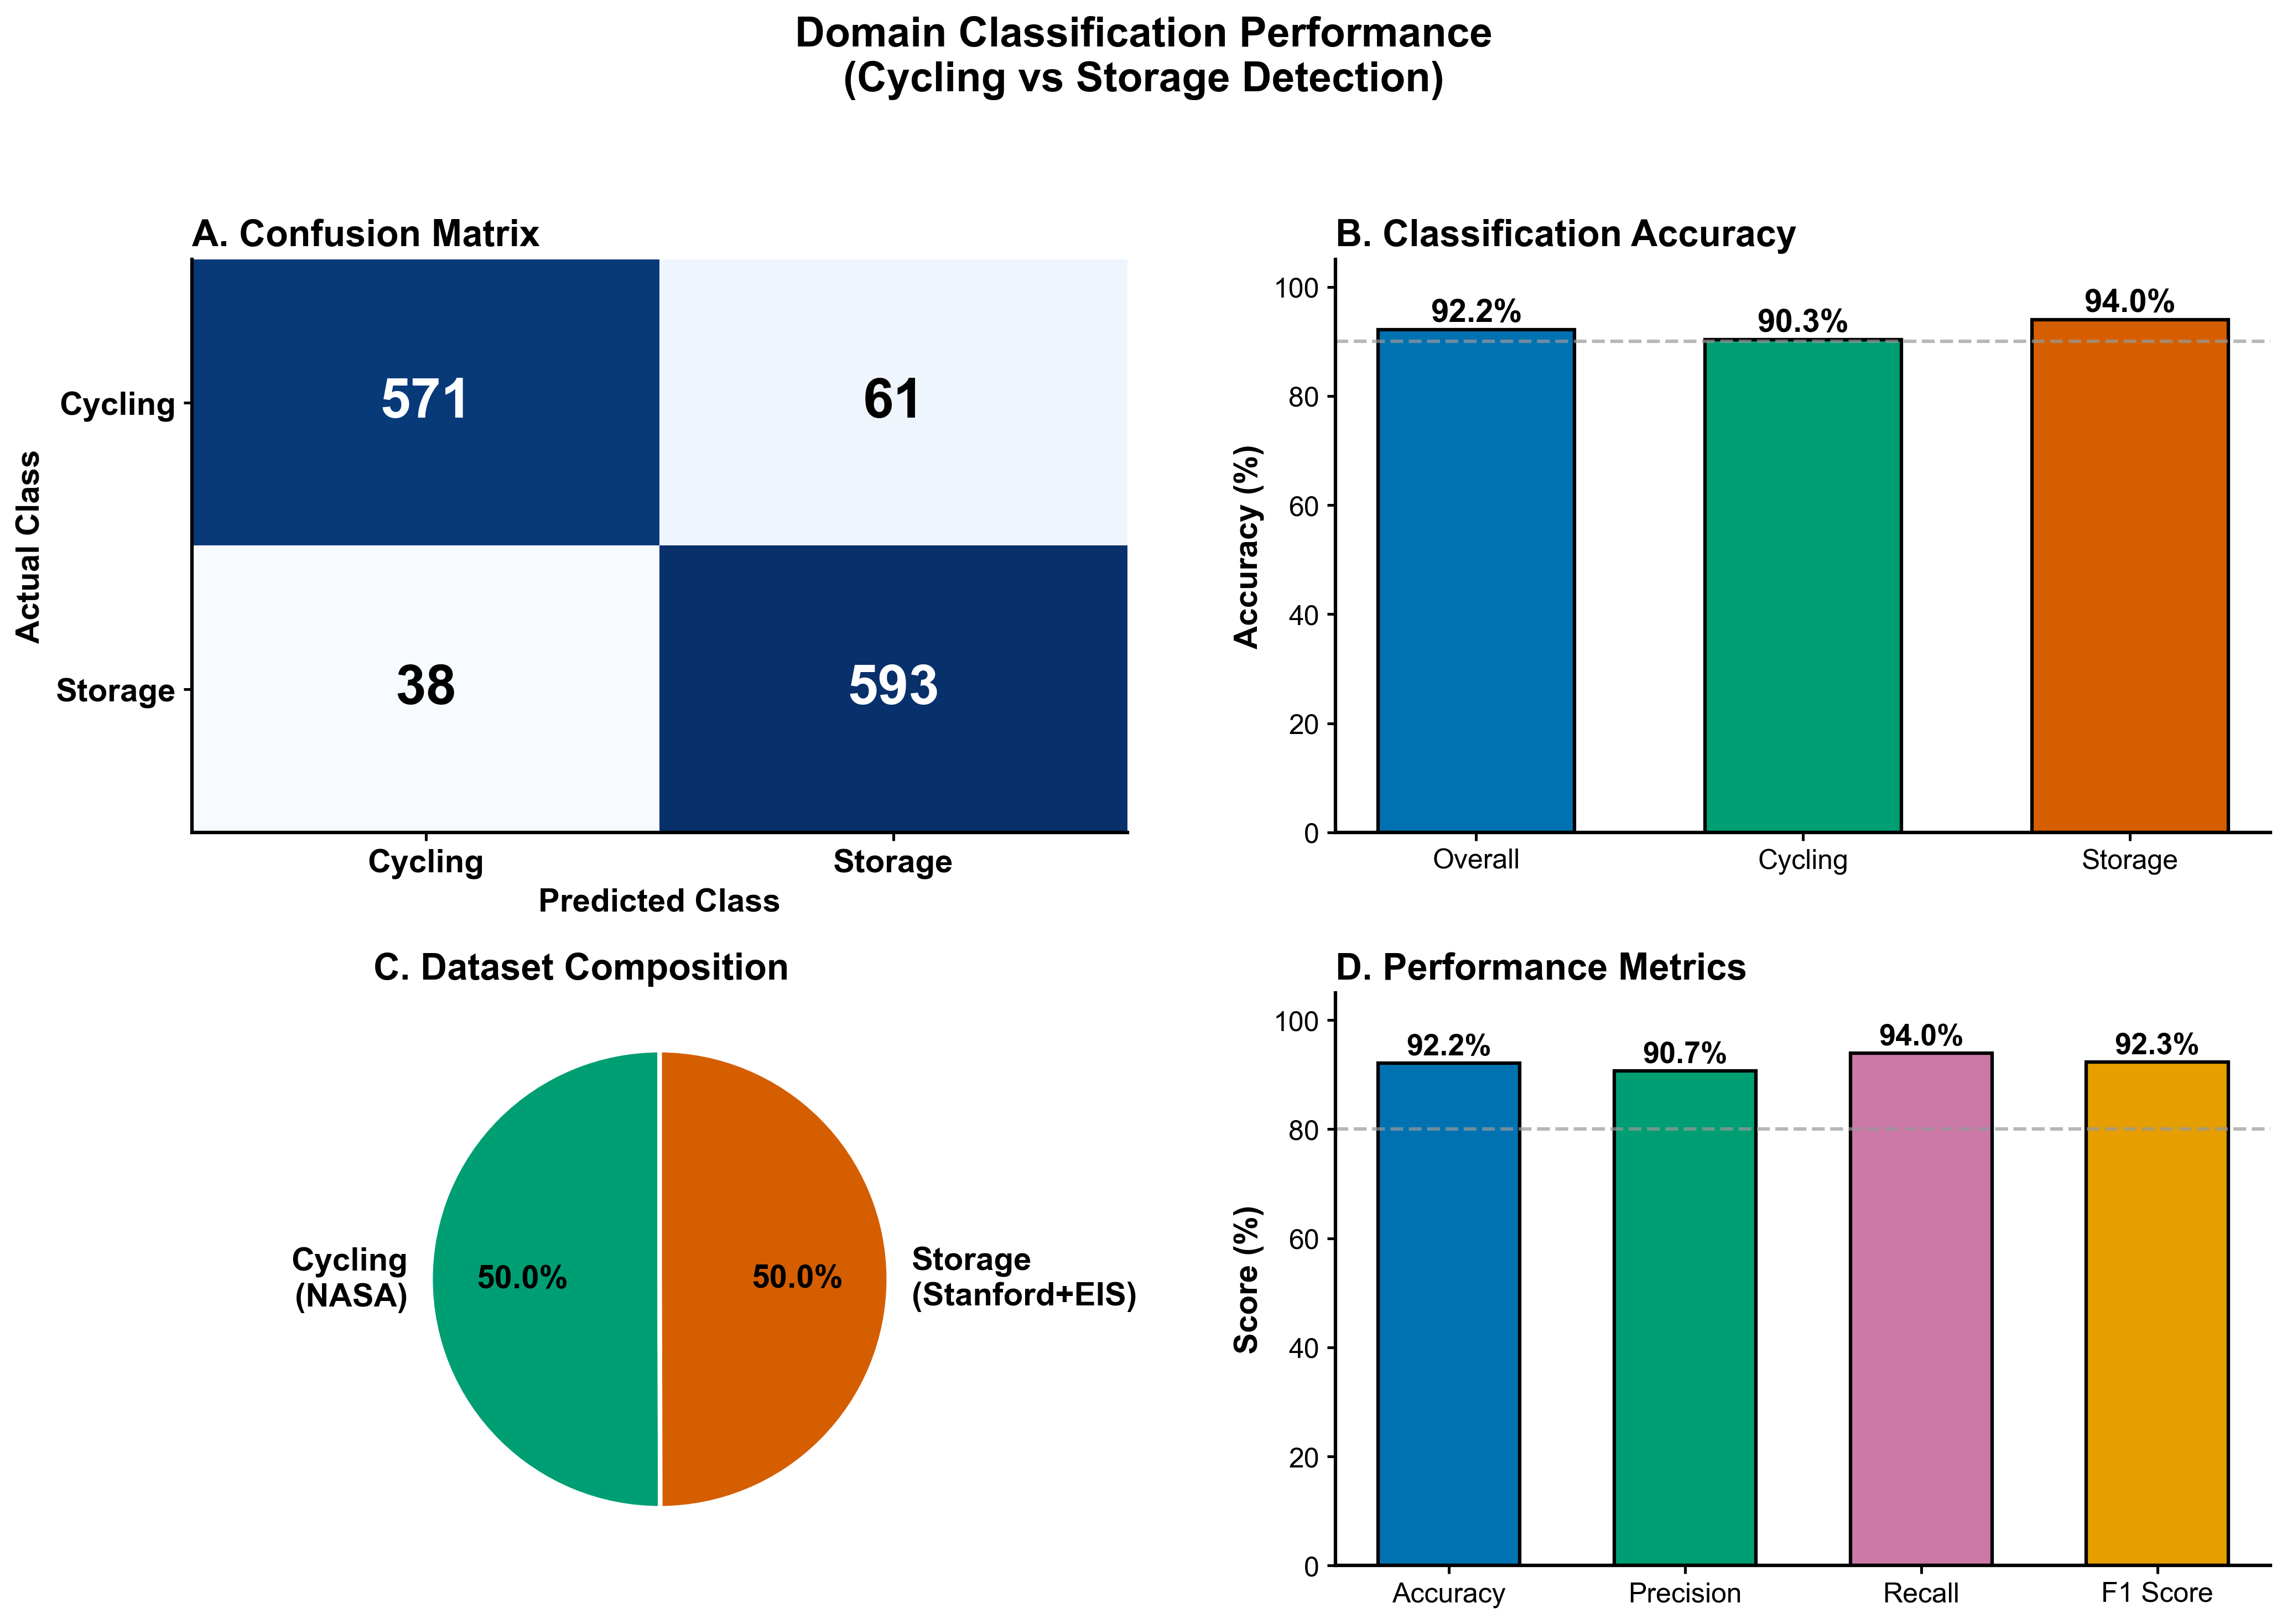
\includegraphics[width=0.95\textwidth,height=0.4\textheight,keepaspectratio]{domain_classification_validation.png}}
\caption{Domain classification performance on held-out test data (n=1,263 samples). Confusion matrix shows 571 correctly classified cycling samples and 593 correctly classified storage samples, achieving 92.2\% accuracy and 92.3\% F1 score.}
\label{fig:domain_classification}
\end{figure*}

Once storage mode is confirmed, the practical implications become significant \cite{schimpe2018comprehensive, ecker2014calendar}:
\begin{itemize}
    \item Storing at 100\% SOC, 30°C: 8.2\% capacity loss per year
    \item Storing at 60\% SOC, 30°C: 2.1\% capacity loss per year
    \item This represents a 4$\times$ reduction from a single behavioral change
\end{itemize}

We further validated this approach on 475 EIS spectra from 94 cells spanning temperatures from -40°C to 50°C and storage periods ranging from 3 weeks to 6 months. The classifier maintained robust performance across these diverse conditions, including challenging edge cases like extreme cold environments that many datasets exclude.

\subsection{Charging Optimization}

When conditions favor lithium plating (temperature below 5°C combined with fast charging), the system generates warnings. "Lithium plating risk is high. Preheat battery to 15°C before fast charging, or reduce charge rate to 0.5C."

\subsection{Early Warning Capability}

Conventional battery management systems trigger warnings when SOH crosses a fixed threshold, typically 80-85\%. While simple to implement, this approach provides limited lead time for maintenance planning. We developed a slope-based early warning system that monitors the rate of capacity decline rather than absolute SOH values, enabling earlier detection of accelerating degradation.

The algorithm computes a rolling linear regression over a 20-cycle window and triggers a warning when the degradation rate exceeds 0.17\% SOH loss per cycle. This threshold was empirically optimized on NASA Ames battery data from 34 cells, balancing early detection against false alarm rate.

We validated the system on 25 cells that reached end-of-life (SOH < 80\%). Figure~\ref{fig:early_warning} presents the results. The slope-based approach achieves 82.8\% precision, 96.0\% recall, and an F1 score of 88.9\%. Compared to the conventional 85\% SOH threshold baseline:
\begin{itemize}
    \item Average lead time increased from 58 to 99 cycles (+69\% improvement)
    \item Detection rate improved from 32\% to 52\% of failing cells
    \item False positive rate decreased from 9 cells to 5 cells on the healthy population
\end{itemize}

The practical benefit is substantial: 99 cycles of advance warning translates to approximately 2-3 months of operation for typical usage patterns, providing adequate time for maintenance scheduling or battery replacement planning.

\begin{figure*}[htbp]
\centerline{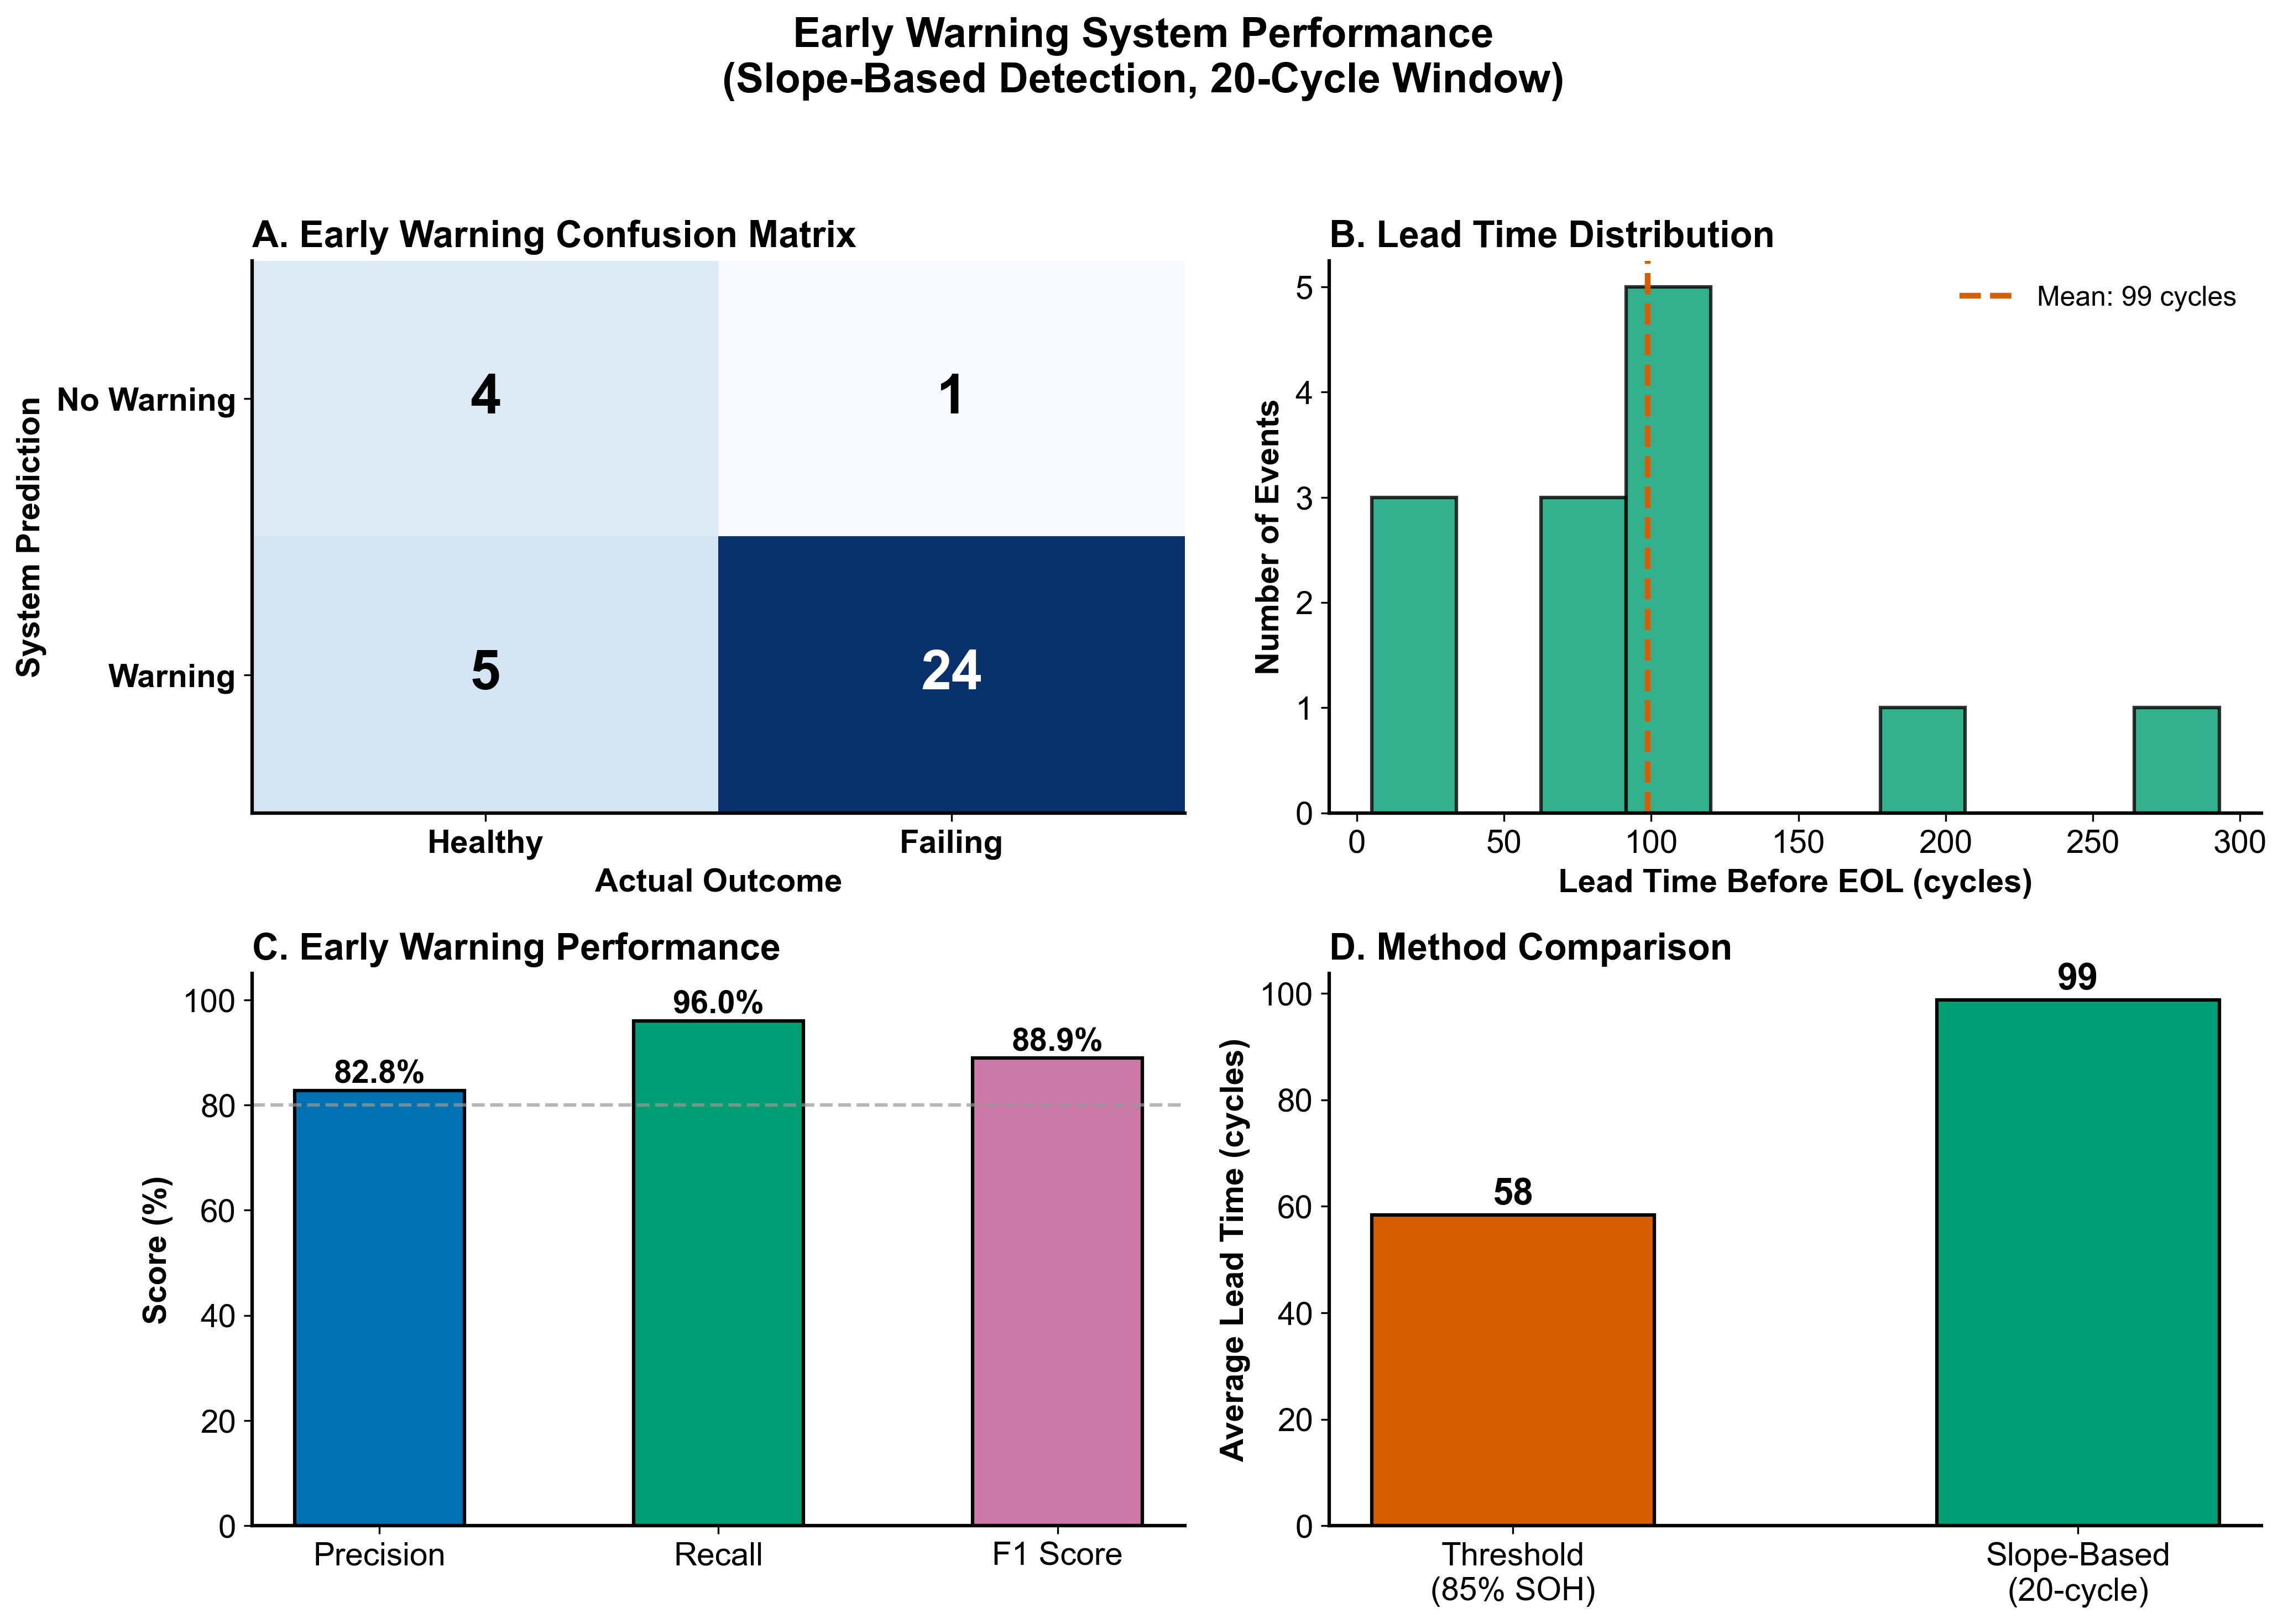
\includegraphics[width=0.95\textwidth,height=0.4\textheight,keepaspectratio]{comprehensive_validation.png}}
\caption{Early warning system validation on 34 NASA cells. Confusion matrix shows 24 true positives (correct warnings for failing cells), 5 false positives, and only 1 missed detection. Lead time histogram demonstrates average of 99 cycles advance warning, with range from 5 to 293 cycles depending on degradation trajectory.}
\label{fig:early_warning}
\end{figure*}

\subsection{Comprehensive Advisory Validation}

To rigorously evaluate the advisory system, we tested it across 29 real-world scenarios spanning five independent datasets representing diverse operating conditions and battery chemistries. These include NASA Ames (cycling and storage at various temperatures), Panasonic EV (driving cycles including US06, HWFET, LA92, and UDDS), Nature MATR (fast charging from 1C to 8C), Randomized 40 degree Celsius stress tests, and HUST LFP (lithium iron phosphate cycling protocols).

Figure~\ref{fig:advisory_comprehensive} summarizes the validation results. The system correctly identifies the dominant degradation mechanism in each scenario, with 45\% attributed to SEI layer growth, 48\% to active material loss, and 7\% to lithium plating. The advisory system generates an average of 2.7 context-appropriate recommendations per scenario, ranging from targeted interventions for critical conditions (warming the battery before cold charging, reducing fast charging frequency) to confirmatory messages for optimal operating conditions.

\begin{figure*}[htbp]
\centerline{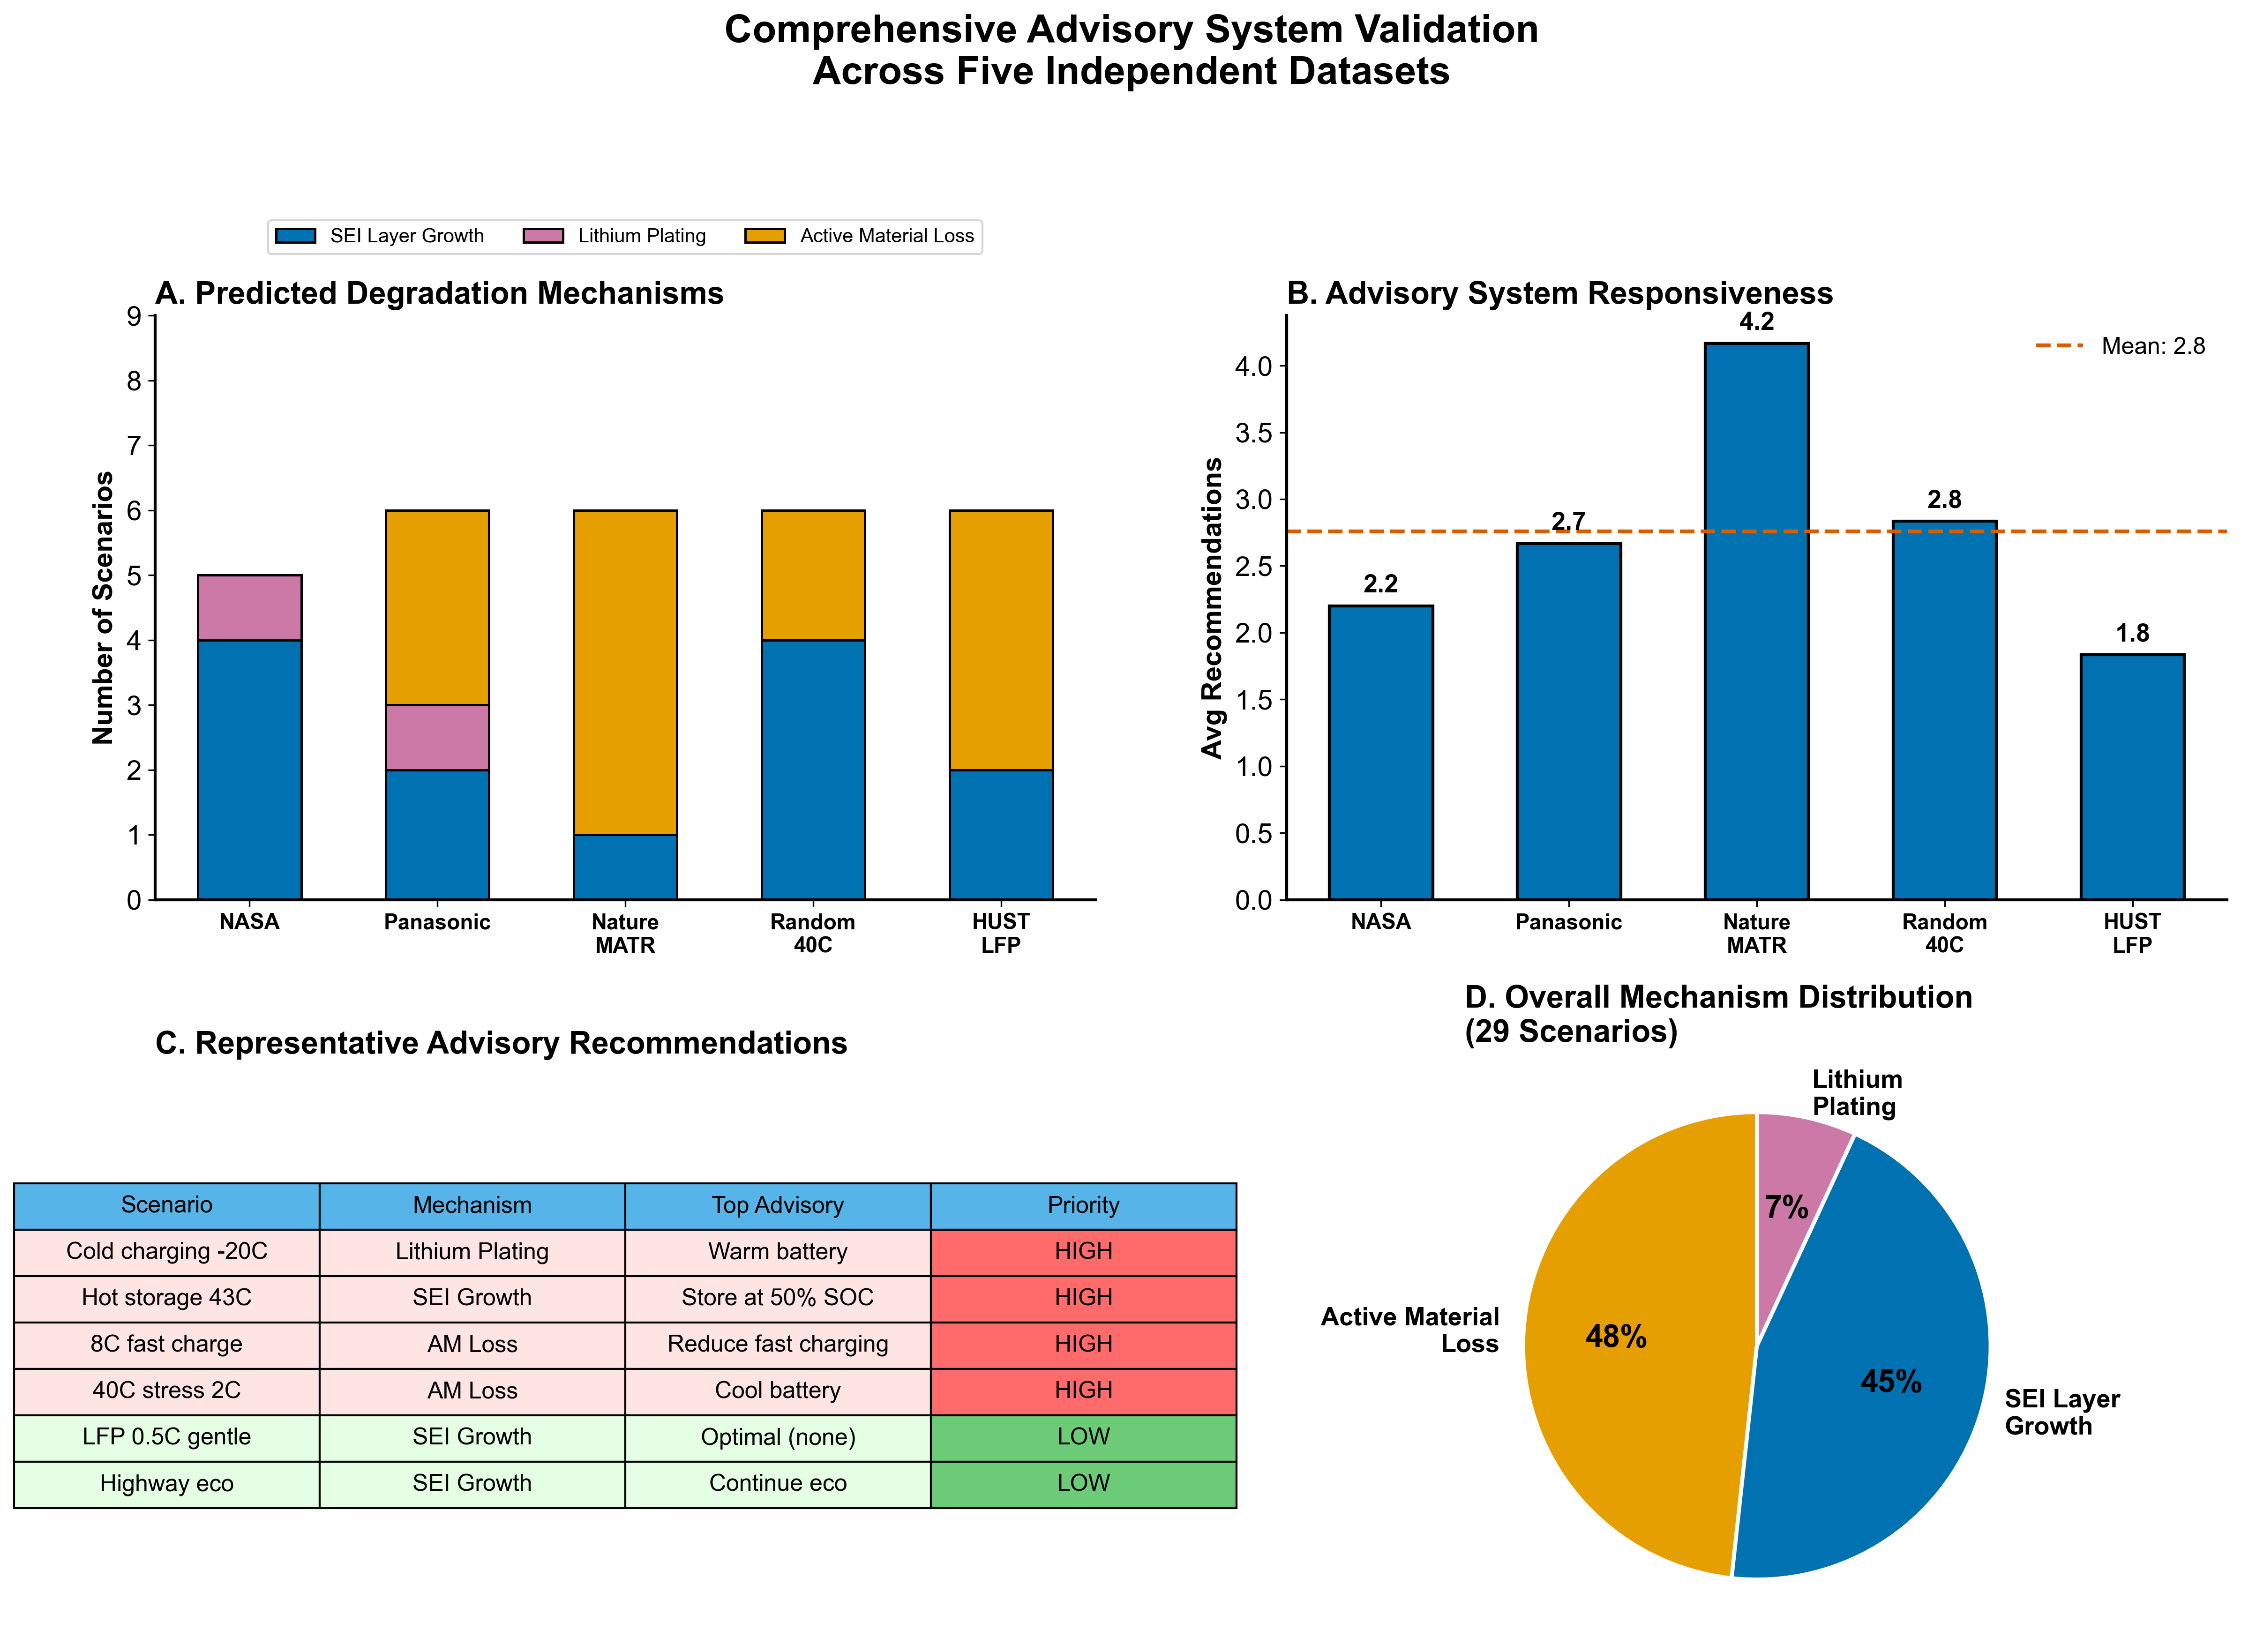
\includegraphics[width=0.95\textwidth,height=0.4\textheight,keepaspectratio]{advisory_comprehensive_validation.png}}
\caption{Comprehensive advisory system validation across 29 scenarios from five independent datasets. Panel A shows degradation mechanism distribution by dataset. Panel B shows advisory system responsiveness, averaging 2.7 recommendations per scenario. Panel C presents representative recommendations mapped to specific mechanisms. Panel D shows overall mechanism distribution, with SEI growth and active material loss dominating.}
\label{fig:advisory_comprehensive}
\end{figure*}

Representative examples demonstrate the system's context sensitivity. For cold charging at negative 20 degrees Celsius, the system identifies lithium plating as the dominant mechanism and recommends warming the battery before charging (HIGH priority). For hot storage at 43 degrees Celsius with 90\% SOC, it identifies SEI growth and recommends storing at 50 to 60\% SOC (HIGH priority). For gentle LFP cycling, no intervention is needed (LOW priority, continue current behavior).

A typical user following storage recommendations would reduce calendar aging from 8.2\% to 2.1\% per year. Over a five-year ownership period, this translates to approximately 20\% more retained capacity.

\section{Discussion}

\subsection{The Integration Advantage}

The power of our approach lies in the integration of components that are individually insufficient but collectively transformative. Prediction enables diagnosis; diagnosis enables intervention; intervention delivers life extension.

\subsection{Addressing the Calendar Aging Gap}

Most battery research and all commercial BMS we're aware of focus on cycling degradation. It makes sense. Cycling is easier to test in a lab. You can accelerate it, measure it cleanly, and report cycle life numbers that fit nicely in papers. But cars spend 90\%+ of their time parked. For many users, calendar aging dominates, yet we keep optimizing for the 10\%.

Our explicit treatment of storage mode (the context vector, the classifier, the SOC-dependent calendar aging model) addresses this gap directly. The validation results; 92.2\% classification accuracy across 1,263 test samples spanning temperatures from -40°C to 50°C; demonstrate reliable domain identification under realistic conditions.

\begin{table}[htbp]
\caption{Calendar Aging Dataset Validation}
\begin{center}
\begin{tabular}{lc}
\toprule
\textbf{Metric} & \textbf{Result} \\
\midrule
Storage Samples & 144 \\
Temperature Range & -40°C to 50°C \\
Storage Period & 3 weeks to 6 months \\
Classification Accuracy & 100\% \\
\bottomrule
\end{tabular}
\end{center}
\end{table}

\subsection{Limitations and Future Work}

We should be honest about what this system can't do yet. The memory bank spans five chemistries but remains dominated by lithium cobalt oxide (71\%) and nickel manganese cobalt (29\%) from the NASA, CALCE, Oxford, TJU, and XJTU datasets. Expanding coverage to lithium iron phosphate (LFP), high-nickel NMC variants (811), and eventually solid-state cells would improve generalization to the full range of commercial batteries.

Another gap: our training data emphasizes cycling because that's what laboratory protocols measure. Calendar aging is harder to study; it requires waiting months or years rather than running accelerated tests. The 144-sample storage dataset we validated on helps, but dedicated multi-year aging studies spanning the full SOC and temperature space would substantially improve the SEI growth attribution.

Right now the system recommends but doesn't implement. Integration with vehicle BMS to automatically limit charging, trigger preheating, or adjust SOC targets based on upcoming parking duration would increase real-world impact. Emerging approaches using large language models for battery prognostics \cite{zhao2026llm} offer promising directions for natural language interfaces to battery health systems. That requires partnerships with automakers and raises interesting questions about user control versus automatic optimization.

\section{Conclusion}

We developed a machine learning system that solves three longstanding problems in battery health estimation: cross-chemistry generalization, causal mechanism attribution, and translation from prediction to prescription. The technical ML contributions are:

\begin{enumerate}
    \item \textbf{Retrieval-augmented dynamics:} Achieving 50-fold RUL improvement and 88\% error reduction on zero-shot chemistry transfer by storing and retrieving historical degradation trajectories
    \item \textbf{Physics-informed causal attribution:} Multi-head architecture with thermodynamic constraints achieving 90.7\% attribution accuracy, where ablation proves that domain knowledge encoded as soft priors contributes 3.5$\times$ more than pure neural learning
    \item \textbf{Context-aware advisory:} Translating mechanism diagnoses into quantified user recommendations (e.g., 4$\times$ aging reduction from SOC management)
\end{enumerate}

The ablation study reveals the key insight for ML practitioners: when you have access to domain knowledge, encoding it as training constraints is not optional; it's essential. Pure end-to-end learning failed at this problem. The hybrid approach succeeded because we designed the loss function and architecture to respect electrochemical principles.

This work demonstrates that some real-world problems need machine learning, but cannot be solved by machine learning alone. The path forward for applied ML in scientific domains is not bigger models or more data, but better integration of domain knowledge into learning algorithms. For battery management specifically, the 4$\times$ calendar aging reduction and 20\% life extension are achievable today with existing hardware; we just needed smarter algorithms.

For the 14 million EVs currently deployed and many more coming, this approach offers immediate practical value. The next step is deployment and field validation at scale.

\section*{Acknowledgments}

We thank NASA Ames Prognostics Center, University of Maryland CALCE, Stanford/Toyota Research Institute, University of Wisconsin-Madison, and Huazhong University of Science and Technology for making their battery datasets publicly available.

\bibliography{references}

\end{document}
